\mode<presentation>
{
  \usetheme{Boadilla}
}

\usepackage[utf8]{inputenc}
\usepackage{booktabs}

\usepackage{minted}
%\usepackage[draft]{minted}
\setminted{frame=single}

\title[Functional programming for humans]{Functional programming for humans}
\subtitle{A gentle, conceptual introduction}
\author{Franklin Chen \\ \url{http://franklinchen.com/}}
\institute{\href{http://www.meetup.com/Pittsburgh-Functional-Programming-Meetup/}{Pittsburgh Functional Programming Meetup}}
\date[October 7,
2015]{\href{http://www.meetup.com/Pittsburgh-Functional-Programming-Meetup/events/224593883/}{October
    7, 2015}}

\subject{Talks}

\AtBeginSection[]
{
  \begin{frame}<beamer>{Outline}
    \tableofcontents[currentsection,subsectionstyle=hide]
  \end{frame}
}

\begin{document}

\maketitle

\begin{abstract}
  We will focus on covering fundamental concepts, making them
  concrete, show patterns and idioms, and how to apply them to work
  flows and application architectures. We will also show how FP is
  related to OO and how to ``think FP'' if you already ``think OO''.

  We will be completely language-inclusive. I've done FP style coding
  in a dozen languages over the years. FP is a state of mind, not a
  language.
\end{abstract}

\begin{frame}
  \titlepage{}
\end{frame}

\section*{Outline}

\begin{frame}{Outline}
  \tableofcontents[subsectionstyle=hide]
\end{frame}

\section{Introduction}

\subsection{Goals}

\begin{frame}{Goals}
  Give enough of an \emph{practical} overview of functional
  programming (FP) to encourage you to
  \begin{itemize}
  \item Learn more, ask questions, become active in the local Pittsburgh FP community.
  \item Do FP!
  \end{itemize}
\end{frame}

\begin{frame}{Non-goals}
  \begin{itemize}
  \item Claim that FP will solve all your problems.
  \item Discuss math and theory behind FP.
  \item Discuss the typed camp of FP.
  \end{itemize}
\end{frame}

\begin{frame}{Topics}
  \begin{itemize}
  \item Functions as used in FP.
  \item Data structures designed for FP.
  \item Comparisons with OO.
  \item The big picture.
  \item Work flows.
  \end{itemize}

  With useful tips and ``secrets''!
\end{frame}

\section{What is functional programming?}

\subsection{Software development is a pain}

\begin{frame}{What real life pain does FP solve?}
  What programmer happiness feels like:
  \begin{itemize}
  \item Self-contained, understandable code.
  \item Testability.
  \item Ease of taking full snapshots of a system; undo/redo.
  \item Reliable reusability of components through composition.
  \item Confidence to perform radical refactoring.
  \item Ease of metaprogramming, domain-specific languages.
  \item Rapid iteration in software development process.
  \item Ease scalability using concurrency and parallelism.
  \end{itemize}
\end{frame}

\subsection{Defining FP}

\begin{frame}{My inclusive definition of FP}
  Doing \emph{most} programming with
  \begin{itemize}
  \item Functions as data.
  \item Pure functions.
  \item Immutable, persistent data structures.
  \end{itemize}

  Some programming languages:
  \begin{itemize}
  \item Have functions that are not quite first-class.
  \item Allow writing non-pure functions by default.
  \item Provide built-in mutable data structures by default.
  \end{itemize}

  \textbf{FP is a state of mind, not a language}.
\end{frame}

\subsection{What is a ``functional language''?}

\begin{frame}{The vague term ``functional language''}
  You can do FP in many languages.

  \begin{alertblock}{There is a catch}
    \begin{itemize}
    \item An FP-tuned standard library and syntax helps \emph{tremendously}.
    \item Quality 3rd-party libraries can fill in gaps.
    \end{itemize}
  \end{alertblock}

  \begin{block}{My recommendations for getting more into FP}
    \begin{itemize}
    \item Start with your current main language: do more FP within
      it.
    \item Pick and commit to learning and using \emph{one} of the
      main FP-optimized languages (next slide).
    \item Learn incrementally by doing and collaborating with others: translate your existing programming experience into FP style.
    \end{itemize}
  \end{block}
\end{frame}

\begin{frame}{Some languages and their level of support for FP}
  (Languages in bold have historical importance.)

  \begin{table}
    \begin{tabular}{| l || l | l | l |}
      \toprule
      & Lower & Moderate & Higher \\
      \midrule
      1957-58 & Fortran & & Lisp \\
      1960 & \textbf{Algol 60} & & \\
      1970-73 & Pascal, C & \textbf{Smalltalk} & \textbf{ML} \\
      1975-78 & Modula-2 & & \textbf{Scheme} \\
      1983-84 & Ada, C++, Objective-C & & Common Lisp \\
      1986-87 & Modula-3, Oberon & Perl & Erlang \\
      1990-91 & & Python & Haskell, SML \\
      1994-95 & Java & Ruby, PHP & OCaml, Racket \\
      1995 & & \textbf{JavaScript} &  \\
      2000-05 & C\#, Visual Basic .NET & & Scala, F\# \\
      2007-09 & Go & & Clojure \\
      2012-14 & & Rust, Swift & Elixir, Elm \\
      \bottomrule
    \end{tabular}
  \end{table}
\end{frame}

\begin{frame}{JavaScript: The Good Part}
  \begin{block}{Why JavaScript is awesome}
    JavaScript has first-class functions.
  \end{block}

  Douglas Crockford:
  \begin{itemize}
  \item 2008: author of book ``JavaScript: The Good Parts''
  \item 2014: spoke on ``JavaScript: The Better Parts''
    \url{http://xahlee.info/js/js_Douglas_Crockford_the_better_parts.html}
    \begin{itemize}
    \item Watch this talk!
    \end{itemize}
  \end{itemize}
\end{frame}

\begin{frame}{You can do non-FP in ``functional languages''}
  If you adopt a ``functional language'':
  \begin{itemize}
  \item You are not ``stuck'' with just pure FP.
  \item ``Functional language'' only means ``functional by default''.
  \item Standard libraries always allow you to do what you did before.
  \item Example: many standard mutable state libraries for Haskell.
  \end{itemize}
\end{frame}

\section{Functions}

% Too low-level, don't want to get bogged down discussing
%\subsection{What is a value?}
%binding
%names, expressions
%environment, closures

\begin{frame}{What is a function in FP?}
  \begin{block}{The core concept for FP}
    \begin{itemize}
    \item Given nontrivial \emph{input} as parameters\ldots{}
    \item \ldots{}a function \emph{communicates} back to caller by \emph{returning} a nontrivial result.
    \end{itemize}
  \end{block}

  FP is about making communication
  \begin{itemize}
  \item Direct; not indirect
  \item Explicit; not implicit
  \end{itemize}

  By making everything explicit, FP allows
  \begin{itemize}
  \item Modeling an entire world as a composite value.
  \item Creating, simulating, testing alternate worlds.
  \item Packaging up a world as a self-contained module.
  \end{itemize}
\end{frame}

\begin{frame}[fragile]{Different communication styles}
  Example: when you call up a pizza shop, how do you order a pizza?

  \begin{table}
    \begin{tabular}{| l || l |}
      \toprule
      & Trivial output \\
      \midrule
      Trivial input
      & \mintinline{js}{order();} \\
      Nontrivial input
      & \mintinline{js}{order([mushrooms, pepperoni]);} \\
      \bottomrule
    \end{tabular}
  \end{table}

  \begin{table}
    \begin{tabular}{| l || l |}
      \toprule
      & Nontrivial output \\
      \midrule
      Trivial input
      & \mintinline{js}{pizzaOrNot = order();} \\
      Nontrivial input
      & \textbf{\mintinline{js}{pizzaOrNot = order([mushrooms, pepperoni]);}} \\
      \bottomrule
    \end{tabular}
  \end{table}

  Depending on communication \emph{context}, each of these is
  a reasonable way to order.
\end{frame}

\begin{frame}{FP: explicit, tight communication style}
  No more
  \begin{itemize}
  \item ``I thought you knew what I wanted on my pizza.''
  \item ``We thought you wanted the pizza delivered where we delivered
    it last time, not where you were calling from.''
\item ``We left the pizza on your porch. It's not our fault someone
  stole it before you opened your door.''
  \end{itemize}

  In FP:
  \begin{itemize}
  \item Every interaction is self-contained, stateless.
  \item Turn input context into parameters.
  \item Turn output context into return values.
  \end{itemize}

  But remember: \textbf{there is no correct communication style}.
\end{frame}

\subsection{Comparing FP with OO}

\begin{frame}[fragile]{OO: methods versus functions}
  In a typical class-based OO language such as Java:
  \begin{itemize}
  \item A \emph{method} is conceptually a \emph{function} with one
    special extra first parameter \mintinline{java}{this}, a reference
    to the ``receiver'' object.
  \end{itemize}

  Imperative programming:
  \begin{table}
    \begin{tabular}{| l || l |}
      \toprule
      & Syntax \\
      \midrule
        Function-based imperative (as in C) & \mintinline{java}{add(myArray, 5);} \\
        Object-based imperative & \mintinline{java}{myArray.add(5);} \\
      \bottomrule
    \end{tabular}
  \end{table}

  So \mintinline{java}{myArray} is mutable, and \mintinline{java}{add}
  \begin{itemize}
  \item returns a trivial result
  \item modifies the state referenced by an input parameter
  \end{itemize}
\end{frame}

\begin{frame}[fragile]{You can do FP in an OO language}
  If you don't mutate your objects, you're doing FP.

  \begin{table}
    \begin{tabular}{| l || l |}
      \toprule
      & Syntax \\
      \midrule
        Function-based FP
      & \mintinline{java}{myNewArray = immutableAdd(myOldArray, 5);} \\
        Object-based FP
      & \mintinline{java}{myNewArray = myOldArray.immutableAdd(5);} \\
      \bottomrule
    \end{tabular}
  \end{table}

  The FP version of \mintinline{java}{add}
  \begin{itemize}
  \item returns a new array
  \item \mintinline{java}{myOldArray} is treated as immutable and not
    modified underneath
  \end{itemize}

  \begin{alertblock}{But, but\ldots isn't this copying around inefficient?}
    \begin{itemize}
    \item Yes, it is inefficient if you use mutable collections designed for
      mutating in place.
    \item No, it is efficient if you use minimal-copying immutable collections
      represented differently (discussed later).
    \end{itemize}
  \end{alertblock}
\end{frame}

\begin{frame}{First-class functions}
  \begin{block}{A popular FP slogan}
    Functions are values!
  \end{block}

  First-class functions are
  \begin{itemize}
  \item Objects existing at runtime.
  \item Can be constructed anywhere.
  \item Can be passed around.
  \item Can be stored like any other data.
  \end{itemize}

  \begin{block}{Fun fact}
    \begin{itemize}
    \item First-class functions invented in the 1920s by Alonzo Church, who
    called his system ``lambda calculus''.
    \item FP is almost 100 years old.
    \end{itemize}
  \end{block}
\end{frame}

\begin{frame}[fragile]{Example of first-class functions in Node.js}
  Redundant version:
  \inputminted{js}{greeters.js}
\end{frame}

\begin{frame}[fragile]{Closures in Node.js}
  Refactor using closures:
  \inputminted{js}{closureGreeters.js}
\end{frame}

\begin{frame}{OO languages recently acquiring first-class functions}
   \begin{itemize}
   \item 2011: C++11
   \item 2014: Java 8
   \end{itemize}

   \begin{block}{Better late than never}
     \begin{itemize}
     \item James Gosling admitted: he wanted to put closures in Java
       20 years ago in 1995 but was under time pressure
     \item Irony: Guy Steele invented the first language with true
       closures (Scheme) in 1975 but was on the Java team
     \end{itemize}
   \end{block}
\end{frame}

\begin{frame}{FP as the simplest special case of OO}
  A tip: if you are used to OO, think of FP as minimalist OO where
  \begin{itemize}
  \item Every object has only one method, let's call it
    \mintinline{java}{run}, taking some number of arguments and
    returning something useful.
  \item Every object is immutable: you can't mutate the fields of your
    object.
  \item There is no inheritance.
  \end{itemize}
\end{frame}

\subsection{Higher-order functions}

\begin{frame}{What is a higher-order function (HOF)?}
  \begin{itemize}
  \item If a function is a worker who does a job and gives you a product\ldots
  \item \ldots{}a higher-order function is a worker who happens to
    delegate or outsource to other workers.
  \end{itemize}

  \begin{itemize}
  \item First-order function: parameters aren't functions.
    \begin{itemize}
    \item Burger flipper uses food as parameters, but no employees.
    \end{itemize}
  \item Higher-order function: parameters may be functions.
    \begin{itemize}
    \item Restaurant owner uses burger flippers as parameters.
    \end{itemize}
  \end{itemize}
\end{frame}

\begin{frame}[fragile]{Example HOF: \mintinline{js}{map} in Node.js}
  \inputminted{js}{mapGreeters.js}
\end{frame}

\begin{frame}{Summary of using functions in FP}
  A function is a one-way pipe flowing between data.
  \begin{itemize}
  \item Always be passing data as parameters.
  \item Always be returning combined, extracted, updated data.
  \item Delegate with higher-order-functions for reusability.
  \end{itemize}
\end{frame}

\section{Data structures}

\begin{frame}{Immutable, persistent data structures}
  Without good data structures, FP is inefficient and clumsy.

  \begin{itemize}
  \item Do not want to copy an entire chunk of data just to change
  a subpart!!
  \item Solution: \emph{structural sharing} of composite data.
  \end{itemize}

  \begin{table}
    \begin{tabular}{| l || l |}
      \toprule
      & Linear data \\
      \midrule
      Mutable & Array \\
      Immutable & Linked list \\
      \bottomrule
    \end{tabular}
  \end{table}
\end{frame}

\subsection{Linked lists}

\begin{frame}[fragile]{Contiguous arrays versus linked lists: code}
  Python built-in arrays versus our simple linked list implementation.

  \inputminted{python}{lists.py}

\href{http://www.pythontutor.com/visualize.html#code=mutableArray+%3D+%5B%22my%22,+%22world%22%5D%0AmutableArrayAlias+%3D+mutableArray+%23+alias+mutableArray%0A%0AmutableArray.insert(0,+%22hello%22%29%0A%0Adef+cons(head,+tail%29%3A%0A++++return+(head,+tail%29%0A++++%0AimmutableList+%3D+cons(%22my%22,+cons(%22world%22,+None%29%29%0AimmutableListAlias+%3D+immutableList%0A%0AnewImmutableList+%3D+cons(%22hello%22,+immutableList%29&mode=display&origin=opt-frontend.js&cumulative=false&heapPrimitives=false&textReferences=false&py=2&rawInputLstJSON=%5B%5D&curInstr=16}{Link to animation on Online Python Tutor}.
\end{frame}

\begin{frame}{Contiguous arrays versus linked lists: visualized}
  \begin{figure}
    % Hack it till it fits!
    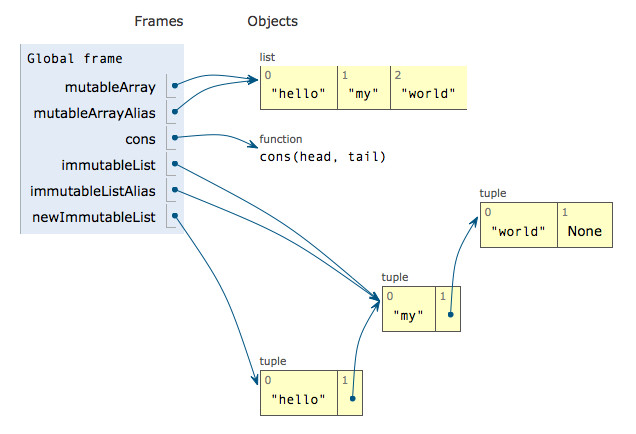
\includegraphics[height=0.7\textheight]{lists.png}
  \end{figure}

  Note that \mintinline{python}{immutableListAlias} is persistent, not lost!
\end{frame}

\begin{frame}[fragile]{Linked list append: code}
  \inputminted{python}{lists2.py}

\href{http://www.pythontutor.com/visualize.html#code=def+cons(head,+tail%29%3A%0A++++return+(head,+tail%29%0A%0Adef+append(list1,+list2%29%3A%0A++++if+list1+is+None%3A%0A++++++++return+list2%0A++++else%3A%0A++++++++head1,+tail1+%3D+list1%0A++++++++return+cons(head1,+append(tail1,+list2%29%29%0A++++++++%0Afirst+%3D+cons(%221%22,+cons(%222%22,+None%29%29%0Asecond+%3D+cons(%223%22,+cons(%224%22,+None%29%29%0Athird+%3D+append(first,+second%29&mode=display&origin=opt-frontend.js&cumulative=false&heapPrimitives=false&textReferences=false&py=2&rawInputLstJSON=%5B%5D&curInstr=37}{Link to animation on Online Python Tutor}.
\end{frame}

\begin{frame}{Linked list append: visualized}
  \begin{figure}
    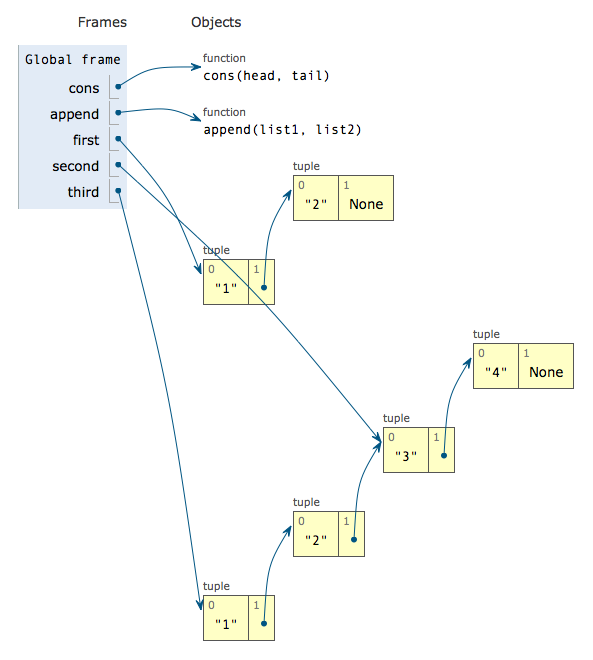
\includegraphics[height=0.8\textheight]{lists2.png}
  \end{figure}
\end{frame}

\begin{frame}{Notes on persistence}
  \begin{block}{The big trick to persistence}
    Copying links as necessary, but not the data pointed to because it
    can be shared.
  \end{block}

  \begin{itemize}
  \item To persist a mutable array, you'd have to make a full copy of
    it to save off to ``defend'' against its being mutated.
  \item Sometimes you want persistence, sometimes you don't: use the
    right tool for the job.
  \end{itemize}
\end{frame}

\begin{frame}{Trees: the single most important persistent data structure}
  The secret to persistent data structures: the tree!
  \begin{itemize}
  \item Dictionaries, sets, arrays, etc.
  \item Structured data that is arbitrarily nested, recursively.
  \item JSON, DOM, anyone?
  \end{itemize}

  \begin{alertblock}{A note on list versus tree}
    \begin{itemize}
    \item In Lisp and other dynamically typed languages, their ``list'' is really a tree.
    \item In typed languages, a list cannot be nested recursively, so
      there are separate tree types.
    \item Untyped languages do provide specialized trees also.
    \end{itemize}
  \end{alertblock}
\end{frame}


\begin{frame}[fragile]{Insertion into a binary tree: code, part 1}
  \inputminted{python}{trees1.py}
\end{frame}

\begin{frame}[fragile]{Insertion into a binary tree: code, part 2}
  \inputminted{python}{trees2.py}

\href{http://www.pythontutor.com/visualize.html#code=def+node(left,+value,+right%29%3A%0A++++return+(left,+value,+right%29%0A%0Adef+insert(x,+tree%29%3A%0A++++if+tree+is+None%3A%0A++++++++return+node(None,+x,+None%29%0A++++else%3A%0A++++++++left,+value,+right+%3D+tree%0A++++++++if+x+%3C+value%3A%0A++++++++++++return+node(insert(x,+left%29,+value,+right%29%0A++++++++elif+x+%3E+value%3A%0A++++++++++++return+node(left,+value,+insert(x,+right%29%29%0A++++++++else%3A%0A++++++++++++return+tree%0A++++++++++++%0Atree1+%3D+node(node(node(None,+1,+None%29,%0A++++++++++++++++++2,%0A++++++++++++++++++node(None,+3,+None%29%29,%0A+++++++++++++5,%0A+++++++++++++node(node(None,+6,+None%29,%0A++++++++++++++++++7,%0A++++++++++++++++++None%29%29++++++++++++%0A++++++++++++++++++%0Atree2+%3D+insert(4,+tree1%29&mode=display&origin=opt-frontend.js&cumulative=false&heapPrimitives=false&textReferences=false&py=2&rawInputLstJSON=%5B%5D&curInstr=64}{Link to animation on Online Python Tutor}.
\end{frame}

\begin{frame}{Insertion into a binary tree: visualized}
  \begin{figure}
    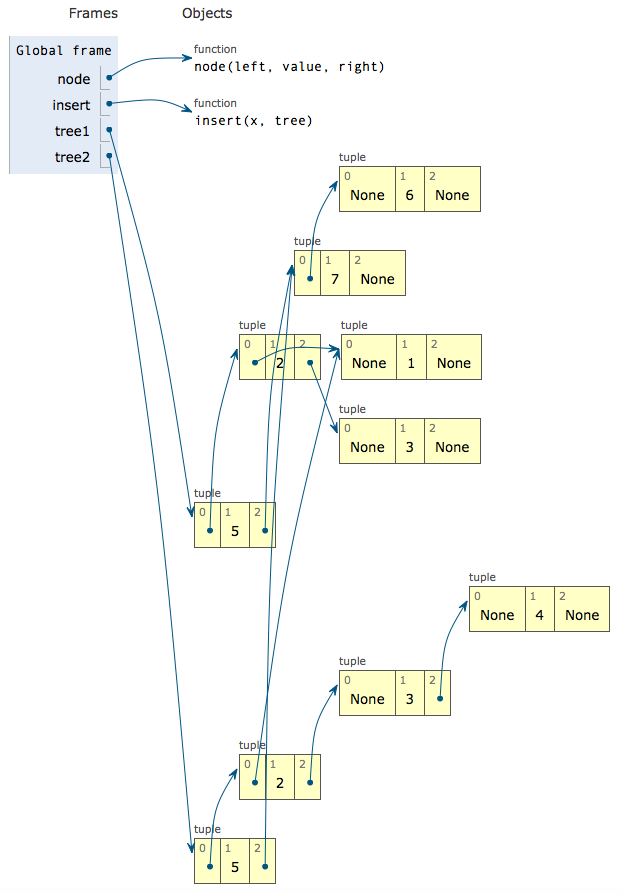
\includegraphics[height=0.8\textheight]{trees.png}
  \end{figure}
\end{frame}

\section{Design patterns and architecture}

\begin{frame}{Functional programming design patterns}
  (Separate talk topic in itself!)

  \begin{itemize}
  \item Yes, there are FP design patterns.
  \item There are some analogues to classic OO design patterns.
    \begin{itemize}
    \item But OO design patterns mostly replaced with use of functions.
    \end{itemize}
  \end{itemize}
\end{frame}

\begin{frame}{Example FP patterns}
  \begin{itemize}
  \item The most-changing argument to a function should be the last argument.
  \item State pattern: pass in old state, returning new state.
  \item Pipeline: pass data from one function to another all
    the way through.
  \item Pass only what is needed into a function, rather than a large
    composite object.
  \item Use the \emph{shape} of data to infer the shape of code of functions
    operating on the data (induction, recursion).
  \item Laziness: avoid evaluating until needed.
  \item Fusion: avoid creating intermediate data structures
    when combining multiple operations on the same data.
  \item Bulk collection patterns: operations such as
    \mintinline{js}{map} and \mintinline{js}{reduce}.
  \item Decorator: higher-order function to turn a function
    into another function.
  \end{itemize}
\end{frame}

\begin{frame}{What about types in FP?}
  Many FP languages strongly emphasize a static type system.

  (A huge topic in itself.)

  \begin{itemize}
  \item Static types enable expression of a huge number of useful
    patterns not available in dynamically typed FP languages.
  \item In turn, some things are easier with dynamic types.
  \end{itemize}
\end{frame}

\begin{frame}{The big picture: architecture}
  \begin{itemize}
  \item One composite global state.
  \item Application transforms one state into another.
  \item Interact with external effectful resources at outermost layer
    possible.
  \item Transform input from world as soon as possible into validated,
    structured data.
  \item Make small functions as generic as possible in input, for
    reuse as modules, libraries.
  \end{itemize}
\end{frame}

\begin{frame}{Example: Elm, pure FP language for front end}
  Elm is a great example of a pure FP architecture for one problem
  domain.

  \begin{itemize}
  \item Check out \href{live Elm demo Web
      apps}{http://elm-lang.org/examples}.
  \item Read the \href{https://github.com/evancz/elm-architecture-tutorial/}{Elm
    architecture tutorial}.
  \end{itemize}
\end{frame}

\section{Work flow}

\begin{frame}{What is it like working using FP?}
  \begin{itemize}
  \item Interactive experimentation with small code snippets in a
    REPL.
  \item Tests easier to write, when state and dependencies minimized.
  \item Modules and type definitions (not classes) as the unit of code organization.
  \item Refactoring easier when code is based on shape of data.
  \end{itemize}
\end{frame}

\section{Conclusion}

\begin{frame}{Conclusion}
  Summary:
  \begin{itemize}
  \item FP has been around, is becoming more mainstream.
  \item Functions are data.
  \item Typical FP patterns and architecture differ from OO.
  \end{itemize}

  \begin{block}{Curious to learn and try more FP?}
    Please fill out the feedback form!
  \end{block}
\end{frame}

\begin{frame}{Slides}
  Slides in source and PDF form:
  \begin{itemize}
  \item \url{https://github.com/FranklinChen/gentle-conceptual-intro-to-fp-for-humans}
  \end{itemize}
\end{frame}

\end{document}
